\documentclass[12pt,]{article}
\usepackage{lmodern}
\usepackage{amssymb,amsmath}
\usepackage{ifxetex,ifluatex}
\usepackage{fixltx2e} % provides \textsubscript
\ifnum 0\ifxetex 1\fi\ifluatex 1\fi=0 % if pdftex
  \usepackage[T1]{fontenc}
  \usepackage[utf8]{inputenc}
\else % if luatex or xelatex
  \ifxetex
    \usepackage{mathspec}
  \else
    \usepackage{fontspec}
  \fi
  \defaultfontfeatures{Ligatures=TeX,Scale=MatchLowercase}
    \setmainfont[]{Times New Roman}
\fi
% use upquote if available, for straight quotes in verbatim environments
\IfFileExists{upquote.sty}{\usepackage{upquote}}{}
% use microtype if available
\IfFileExists{microtype.sty}{%
\usepackage{microtype}
\UseMicrotypeSet[protrusion]{basicmath} % disable protrusion for tt fonts
}{}
\usepackage[margin=2.54cm]{geometry}
\usepackage{hyperref}
\hypersetup{unicode=true,
            pdftitle={Changes in Land Use between 1990 and 2014},
            pdfauthor={Rebecca Marx},
            pdfborder={0 0 0},
            breaklinks=true}
\urlstyle{same}  % don't use monospace font for urls
\usepackage{color}
\usepackage{fancyvrb}
\newcommand{\VerbBar}{|}
\newcommand{\VERB}{\Verb[commandchars=\\\{\}]}
\DefineVerbatimEnvironment{Highlighting}{Verbatim}{commandchars=\\\{\}}
% Add ',fontsize=\small' for more characters per line
\usepackage{framed}
\definecolor{shadecolor}{RGB}{248,248,248}
\newenvironment{Shaded}{\begin{snugshade}}{\end{snugshade}}
\newcommand{\KeywordTok}[1]{\textcolor[rgb]{0.13,0.29,0.53}{\textbf{#1}}}
\newcommand{\DataTypeTok}[1]{\textcolor[rgb]{0.13,0.29,0.53}{#1}}
\newcommand{\DecValTok}[1]{\textcolor[rgb]{0.00,0.00,0.81}{#1}}
\newcommand{\BaseNTok}[1]{\textcolor[rgb]{0.00,0.00,0.81}{#1}}
\newcommand{\FloatTok}[1]{\textcolor[rgb]{0.00,0.00,0.81}{#1}}
\newcommand{\ConstantTok}[1]{\textcolor[rgb]{0.00,0.00,0.00}{#1}}
\newcommand{\CharTok}[1]{\textcolor[rgb]{0.31,0.60,0.02}{#1}}
\newcommand{\SpecialCharTok}[1]{\textcolor[rgb]{0.00,0.00,0.00}{#1}}
\newcommand{\StringTok}[1]{\textcolor[rgb]{0.31,0.60,0.02}{#1}}
\newcommand{\VerbatimStringTok}[1]{\textcolor[rgb]{0.31,0.60,0.02}{#1}}
\newcommand{\SpecialStringTok}[1]{\textcolor[rgb]{0.31,0.60,0.02}{#1}}
\newcommand{\ImportTok}[1]{#1}
\newcommand{\CommentTok}[1]{\textcolor[rgb]{0.56,0.35,0.01}{\textit{#1}}}
\newcommand{\DocumentationTok}[1]{\textcolor[rgb]{0.56,0.35,0.01}{\textbf{\textit{#1}}}}
\newcommand{\AnnotationTok}[1]{\textcolor[rgb]{0.56,0.35,0.01}{\textbf{\textit{#1}}}}
\newcommand{\CommentVarTok}[1]{\textcolor[rgb]{0.56,0.35,0.01}{\textbf{\textit{#1}}}}
\newcommand{\OtherTok}[1]{\textcolor[rgb]{0.56,0.35,0.01}{#1}}
\newcommand{\FunctionTok}[1]{\textcolor[rgb]{0.00,0.00,0.00}{#1}}
\newcommand{\VariableTok}[1]{\textcolor[rgb]{0.00,0.00,0.00}{#1}}
\newcommand{\ControlFlowTok}[1]{\textcolor[rgb]{0.13,0.29,0.53}{\textbf{#1}}}
\newcommand{\OperatorTok}[1]{\textcolor[rgb]{0.81,0.36,0.00}{\textbf{#1}}}
\newcommand{\BuiltInTok}[1]{#1}
\newcommand{\ExtensionTok}[1]{#1}
\newcommand{\PreprocessorTok}[1]{\textcolor[rgb]{0.56,0.35,0.01}{\textit{#1}}}
\newcommand{\AttributeTok}[1]{\textcolor[rgb]{0.77,0.63,0.00}{#1}}
\newcommand{\RegionMarkerTok}[1]{#1}
\newcommand{\InformationTok}[1]{\textcolor[rgb]{0.56,0.35,0.01}{\textbf{\textit{#1}}}}
\newcommand{\WarningTok}[1]{\textcolor[rgb]{0.56,0.35,0.01}{\textbf{\textit{#1}}}}
\newcommand{\AlertTok}[1]{\textcolor[rgb]{0.94,0.16,0.16}{#1}}
\newcommand{\ErrorTok}[1]{\textcolor[rgb]{0.64,0.00,0.00}{\textbf{#1}}}
\newcommand{\NormalTok}[1]{#1}
\usepackage{longtable,booktabs}
\usepackage{graphicx,grffile}
\makeatletter
\def\maxwidth{\ifdim\Gin@nat@width>\linewidth\linewidth\else\Gin@nat@width\fi}
\def\maxheight{\ifdim\Gin@nat@height>\textheight\textheight\else\Gin@nat@height\fi}
\makeatother
% Scale images if necessary, so that they will not overflow the page
% margins by default, and it is still possible to overwrite the defaults
% using explicit options in \includegraphics[width, height, ...]{}
\setkeys{Gin}{width=\maxwidth,height=\maxheight,keepaspectratio}
\IfFileExists{parskip.sty}{%
\usepackage{parskip}
}{% else
\setlength{\parindent}{0pt}
\setlength{\parskip}{6pt plus 2pt minus 1pt}
}
\setlength{\emergencystretch}{3em}  % prevent overfull lines
\providecommand{\tightlist}{%
  \setlength{\itemsep}{0pt}\setlength{\parskip}{0pt}}
\setcounter{secnumdepth}{5}
% Redefines (sub)paragraphs to behave more like sections
\ifx\paragraph\undefined\else
\let\oldparagraph\paragraph
\renewcommand{\paragraph}[1]{\oldparagraph{#1}\mbox{}}
\fi
\ifx\subparagraph\undefined\else
\let\oldsubparagraph\subparagraph
\renewcommand{\subparagraph}[1]{\oldsubparagraph{#1}\mbox{}}
\fi

%%% Use protect on footnotes to avoid problems with footnotes in titles
\let\rmarkdownfootnote\footnote%
\def\footnote{\protect\rmarkdownfootnote}

%%% Change title format to be more compact
\usepackage{titling}

% Create subtitle command for use in maketitle
\providecommand{\subtitle}[1]{
  \posttitle{
    \begin{center}\large#1\end{center}
    }
}

\setlength{\droptitle}{-2em}

  \title{Changes in Land Use between 1990 and 2014}
    \pretitle{\vspace{\droptitle}\centering\huge}
  \posttitle{\par}
  \subtitle{\url{https://github.com/RsMarx/Ag_Forest_Data_Final-}}
  \author{Rebecca Marx}
    \preauthor{\centering\large\emph}
  \postauthor{\par}
    \date{}
    \predate{}\postdate{}
  

\begin{document}
\maketitle
\begin{abstract}
This study uses data spanning 264 countries to explore the causes and
impacts of changes in land use from 1990 to 2014. It confirms a slight
trend of decreasing levels of forest cover globally which can be
explained, in part, by an increase in agriculture cover. In addition to
addressing the impacts of agricultural expansion on forest cover, the
study considers the roles that electricity access and renewable energy
have to play in forest cover trends. Finally, a clear link is drawn
between increases in agriculture cover, decreases in forest cover, and
increases in emissions of methane and nitrous oxide. The study was
conducted using a series of linear mixed-effect models with country as a
random effect, as well as tests to confirm there are no problems with
multicollinearity. While the study looks at trends across all countries
in the data set, it also highlights the chain of causes and impacts of
land cover change in five countries in five distinct regions. A set of
graphs illustrate the differences and similarities of individual country
experiences. Overall, the study is a helpful resource for continuing the
discussion around protecting forests from conversion to other land uses,
such as agriculture.
\end{abstract}

\newpage

\tableofcontents  \newpage
\listoftables  \newpage
\listoffigures  \newpage

\textless{}Note: set up autoreferencing for figures and tables in your
document\textgreater{}

\section{Research Question and
Rationale}\label{research-question-and-rationale}

As the global population continues to grow and require more food and
fuel resources, deforestation trends are expected to accelerate.
Deforestation can be problematic as forests provide ecosystem services
such as carbon storage, nutrient cycling, water filtration, and wildlife
habitat. Agriculture is one of the most commonly sited drivers of
deforestation, in addition to being a source of emissions. Given that
forest and agriculture can be contending land uses, this research
examines the relationship between agriculture and forest as land uses
and, more broadly, explores the causes and impacts of changes in land
use.

This research looks at the trends and tradeoffs in land use across
countries from 1990 -- 2014. Primary questions include:

\begin{itemize}
\tightlist
\item
  Is there a relationship between the percentage of land area dedicated
  to forest versus agricultural in countries?
\item
  Is there a relationship between land uses (agriculture or forest) and
  levels of CO2, methane, and nitrous oxide emissions?
\item
  Is there a relationship between access to electricity or renewable
  electricity output and the percentage of land dedicated to forestry
  versus agriculture?
\end{itemize}

Emissions variables are included becasue emissions are expected to
increase if agricultural activities increase. Electricity data are
included because biomass from forests can be a source of fuel for those
who do not have access to electricity. Furthermore, biofuel produced
from wood chips and crops is considered a source of renewable energy.

The research utilizes a data set from the World Bank that has 135
environment-related variables for 264 countries. I have narrowed the
environment variable down to 7 that are relevant to land use. Although
the full data set dates back to 1960, I have limited to the time scope
of the analysis to between 1990 and 2014 because those are the dates for
which all data is available.

\newpage

\section{Dataset Information}\label{dataset-information}

\subsection{Database Information}\label{database-information}

Data were collected from the World Bank website. More information can be
found here: \url{https://data.worldbank.org/topic/environment}

Data were downloaded as a full data set called
``API\_6\_DS2\_en\_csv\_v2\_10518155''. The csv file was saved as
``WorldBank\_Raw\_4.8.19''.

Variables from among the raw data set were selected to be used in the
data set analysed. Only 7 of a possible 135 environment-related
variables were retained in the processed data. This csv file was saved
as {[}``WorldBank\_Processed''; ``WorldBank\_Spread'' or
``WB\_Spread''{]}.

\subsection{Data Content Information}\label{data-content-information}

\textbf{Country}: Originally named ``Country.Name'', the Country
variable includes 264 countries.

\textbf{Year}: The Year variable was originally spread horizontally from
1960 -- 2018. The years were gathered in to one column named ``Year''
and formatted as a date.

\textbf{Forest}: The Forest variable was originally named ``Forest area
(\% of land area)''. Its data range is 1990 -- 2016.

\textbf{Agriculture}: The Agriculture variable was originally named
``Agriculture land (\% of land area). Its data range is from 1961 --
2018.

\textbf{Ag.Methane}: The Ag.Methane variable was originally named
``Agriculture methane emissions (thousand metric tons of CO2
equivalent). Its data range is 1970 -- 2008.

\textbf{Ag.NO2}: The Ag.NO2 variable was originally named ``Agriculture
nitrous oxide emissions (thousand metric tons of CO2 equivalent). Its
data range is 1970 -- 2008.

\textbf{CO2Emissions}: The CO2Emissions variable was originally named
``CO2 emissions (kt). Its data range is 1960 -- 2014.

\textbf{ElectricityAccess}: The ElectricityAccess variable was
originally named ``Access to electricity (\% of total population). Data
range is 1990 -- 2016.

\textbf{RenewableElectricity}: The RenewableElectricity variable was
originally named ``Renewable electricity output (\% of total electricity
output). Its data range is 1990 -- 2015.

\subsection{Naming conventions and file
formats}\label{naming-conventions-and-file-formats}

The files are named according to the following convention:
databasename\_datatype\_details\_stage.format where: Files are named
according to the following naming convention: \textbf{databasename}
refers to the database from where the data originated \textbf{details}
are additional descriptive details related to the stage of data
wrangling \textbf{stage} refers to the stage in data management
pipelines (e.g., raw or processed) \textbf{format} is a non-proprietary
file format (e.g., .csv, .txt)

\textbf{Additional Information and Support}

For more information, please contact the data assembler, \textbf{Rebecca
Marx}
(\href{mailto:rebecca.marx@duke.edu}{\nolinkurl{rebecca.marx@duke.edu}})

\textbf{Summary of Data Structure}

\begin{longtable}[]{@{}lll@{}}
\caption{\label{tab:table} World Bank Land Cover Data
Summary}\tabularnewline
\toprule
Indicator & Units & Data Structure\tabularnewline
\midrule
\endfirsthead
\toprule
Indicator & Units & Data Structure\tabularnewline
\midrule
\endhead
Country & Name & Factor\tabularnewline
Indicator.Code & Abbrv & Factor\tabularnewline
Year & YYYY & Date\tabularnewline
ElectricityAccess & \% Total Population & Numeric\tabularnewline
Agriculture & \% Land Area & Numeric\tabularnewline
Ag.Methane & Thousand Metric Tons of CO2 Equivalent &
Numeric\tabularnewline
Ag.N2O & Thousand Metric Tons of CO2 Equivalent & Numeric\tabularnewline
CO2Emissions & Kilotons & Numeric\tabularnewline
Forest & \% Land Area & Numeric\tabularnewline
RenewableElectricity & \% Total Output & Numeric\tabularnewline
\bottomrule
\end{longtable}

\newpage

\section{Exploratory Data Analysis and
Wrangling}\label{exploratory-data-analysis-and-wrangling}

\subsection{Data Wrangling}\label{data-wrangling}

Wrangling the data required multiple operations. First, I used the
filter function to select only 7 of a possible 135 variables in the data
set. Since the data set was arranged with the years going horizontally,
I then had to gather the years in to one column, and create a new column
called ``Level'' that contained the values recorded for each variable in
each year. Afterward, I used spread to make each environmental variable
its own column. I had to remove an ``X'' from in front of the Year, and
format the Year as a date. I also had to update column names because
they were very long. For certain tests, I had to drop na from the data
set.

\begin{Shaded}
\begin{Highlighting}[]
\NormalTok{World_Bank_Master <-}\KeywordTok{read.csv}\NormalTok{(}\StringTok{"../Raw/WorldBank_Raw2_4.8.19.csv"}\NormalTok{)}

\CommentTok{#Data Subset}
\NormalTok{World_Bank_Filter <-}\StringTok{ }\KeywordTok{filter}\NormalTok{(World_Bank_Master, }
\NormalTok{Indicator.Name }\OperatorTok{==}\StringTok{ "Forest area (% of land area)"} \OperatorTok{|}\StringTok{ }
\NormalTok{Indicator.Name }\OperatorTok{==}\StringTok{ "Agricultural land (% of land area)"} \OperatorTok{|}\StringTok{ }
\NormalTok{Indicator.Name }\OperatorTok{==}\StringTok{ "Access to electricity (% of population)"} \OperatorTok{|}\StringTok{ }
\NormalTok{Indicator.Name }\OperatorTok{==}\StringTok{ "Renewable electricity output (% of total electricity output)"} \OperatorTok{|}\StringTok{ }
\NormalTok{Indicator.Name }\OperatorTok{==}\StringTok{ "CO2 emissions (kt)"} \OperatorTok{|}\StringTok{ }
\NormalTok{Indicator.Name }\OperatorTok{==}\StringTok{ "Agricultural nitrous oxide emissions (thousand metric tons of CO2 equivalent)"} \OperatorTok{|}\StringTok{ }\NormalTok{Indicator.Name }\OperatorTok{==}\StringTok{ "Agricultural methane emissions (thousand metric tons of CO2 equivalent)"}\NormalTok{)}

\NormalTok{WorldBank_Gather <-}\StringTok{ }\KeywordTok{gather}\NormalTok{(World_Bank_Filter, }\StringTok{"Year"}\NormalTok{, }\StringTok{"Level"}\NormalTok{, X1960}\OperatorTok{:}\NormalTok{X2018)}

\NormalTok{WorldBank_Gather <-}\StringTok{ }\KeywordTok{select}\NormalTok{(WorldBank_Gather, }\OperatorTok{-}\NormalTok{Indicator.Code)}

\NormalTok{WorldBank_Spread <-}\StringTok{  }\KeywordTok{spread}\NormalTok{(WorldBank_Gather, Indicator.Name, Level)}

\CommentTok{#Format as character }
\NormalTok{WorldBank_Spread}\OperatorTok{$}\NormalTok{Year <-}\StringTok{ }\KeywordTok{as.character}\NormalTok{(WorldBank_Spread}\OperatorTok{$}\NormalTok{Year)}

\CommentTok{#create string}
\NormalTok{WB_String <-}\StringTok{ }\KeywordTok{substr}\NormalTok{(WorldBank_Spread}\OperatorTok{$}\NormalTok{Year, }\DecValTok{2}\NormalTok{, }\DecValTok{5}\NormalTok{)}

\CommentTok{#Get rid of X in date}
\NormalTok{WorldBank_Spread}\OperatorTok{$}\NormalTok{Year =}\StringTok{ }\NormalTok{WB_String}

\CommentTok{#Format as date}
\CommentTok{#WB_Fixed$Year <- as.Date(WB_Fixed$Year)}
\NormalTok{WorldBank_Spread}\OperatorTok{$}\NormalTok{Year <-}\StringTok{ }\KeywordTok{as.Date}\NormalTok{(WorldBank_Spread}\OperatorTok{$}\NormalTok{Year, }\DataTypeTok{format =} \StringTok{"%Y"}\NormalTok{) }

\CommentTok{#Change column names }
\KeywordTok{names}\NormalTok{(WorldBank_Spread) <-}\StringTok{ }\KeywordTok{c}\NormalTok{(}\StringTok{"Country"}\NormalTok{, }\StringTok{"Indicator.Code"}\NormalTok{, }\StringTok{"Year"}\NormalTok{, }
\StringTok{"ElectricityAccess"}\NormalTok{, }\StringTok{"Agriculture"}\NormalTok{, }\StringTok{"Ag.Methane"}\NormalTok{, }\StringTok{"Ag.N2O"}\NormalTok{, }
\StringTok{"CO2Emissions"}\NormalTok{, }\StringTok{"Forest"}\NormalTok{, }\StringTok{"RenewableElectricity"}\NormalTok{)}

\CommentTok{#Save processed file }
\CommentTok{#write.csv(WorldBank_Spread, }
\CommentTok{#row.names = FALSE, file = "../Processed/WorldBank_Processed.csv")}
   
\NormalTok{Five_Countries <-}\StringTok{ }\KeywordTok{filter}\NormalTok{(WorldBank_Spread, Country }\OperatorTok{==}\StringTok{ "Brazil"} \OperatorTok{|}\StringTok{ }
\NormalTok{Country }\OperatorTok{==}\StringTok{ "Kenya"} \OperatorTok{|}\StringTok{ }\NormalTok{Country }\OperatorTok{==}\StringTok{ "Spain"} \OperatorTok{|}\StringTok{ }
\NormalTok{Country }\OperatorTok{==}\StringTok{ "Indonesia"} \OperatorTok{|}\StringTok{ }\NormalTok{Country }\OperatorTok{==}\StringTok{ "Canada"}\NormalTok{)}

\NormalTok{WB_Spread <-}\StringTok{ }\NormalTok{WorldBank_Spread }\OperatorTok\StringTok{ }
\StringTok{  }\NormalTok{na.exclude }\CommentTok{#check if I need this for my tests}

\NormalTok{WB_Spread2 <-}\StringTok{ }\NormalTok{WorldBank_Spread }\OperatorTok\StringTok{ }
\StringTok{  }\NormalTok{na.exclude}

\NormalTok{WB_Brazil <-}\StringTok{ }\KeywordTok{filter}\NormalTok{(WorldBank_Spread, Country }\OperatorTok{==}\StringTok{ "Brazil"}\NormalTok{)}
\end{Highlighting}
\end{Shaded}

\begin{verbatim}
\end{verbatim}

\subsection{Data Exploration}\label{data-exploration}

After the data was wrangled into a format that would function well with
my intended R operations, I was able to begin exploring the data set.

\begin{Shaded}
\begin{Highlighting}[]
\CommentTok{#5+ lines of summary }

\KeywordTok{colnames}\NormalTok{(WorldBank_Spread)}
\end{Highlighting}
\end{Shaded}

\begin{verbatim}
##  [1] "Country"              "Indicator.Code"       "Year"                
##  [4] "ElectricityAccess"    "Agriculture"          "Ag.Methane"          
##  [7] "Ag.N2O"               "CO2Emissions"         "Forest"              
## [10] "RenewableElectricity"
\end{verbatim}

\begin{Shaded}
\begin{Highlighting}[]
\KeywordTok{str}\NormalTok{(WorldBank_Spread)}
\end{Highlighting}
\end{Shaded}

\begin{verbatim}
## 'data.frame':    15576 obs. of  10 variables:
##  $ Country             : Factor w/ 264 levels "Afghanistan",..: 1 1 1 1 1 1 1 1 1 1 ...
##  $ Indicator.Code      : Factor w/ 264 levels "ABW","AFG","AGO",..: 2 2 2 2 2 2 2 2 2 2 ...
##  $ Year                : Date, format: "1960-04-16" "1961-04-16" ...
##  $ ElectricityAccess   : num  NA NA NA NA NA NA NA NA NA NA ...
##  $ Agriculture         : num  NA 57.7 57.8 57.9 58 ...
##  $ Ag.Methane          : num  NA NA NA NA NA NA NA NA NA 0 ...
##  $ Ag.N2O              : num  NA NA NA NA NA NA NA NA NA 0 ...
##  $ CO2Emissions        : num  414 491 689 708 840 ...
##  $ Forest              : num  NA NA NA NA NA NA NA NA NA NA ...
##  $ RenewableElectricity: num  NA NA NA NA NA NA NA NA NA NA ...
\end{verbatim}

\begin{Shaded}
\begin{Highlighting}[]
\KeywordTok{class}\NormalTok{(WorldBank_Spread}\OperatorTok{$}\NormalTok{Year)}
\end{Highlighting}
\end{Shaded}

\begin{verbatim}
## [1] "Date"
\end{verbatim}

\begin{Shaded}
\begin{Highlighting}[]
\KeywordTok{dim}\NormalTok{(WorldBank_Spread)}
\end{Highlighting}
\end{Shaded}

\begin{verbatim}
## [1] 15576    10
\end{verbatim}

\begin{Shaded}
\begin{Highlighting}[]
\KeywordTok{head}\NormalTok{(WorldBank_Spread)}
\end{Highlighting}
\end{Shaded}

\begin{verbatim}
##       Country Indicator.Code       Year ElectricityAccess Agriculture
## 1 Afghanistan            AFG 1960-04-16                NA          NA
## 2 Afghanistan            AFG 1961-04-16                NA    57.74592
## 3 Afghanistan            AFG 1962-04-16                NA    57.83782
## 4 Afghanistan            AFG 1963-04-16                NA    57.91441
## 5 Afghanistan            AFG 1964-04-16                NA    58.01091
## 6 Afghanistan            AFG 1965-04-16                NA    58.01397
##   Ag.Methane Ag.N2O CO2Emissions Forest RenewableElectricity
## 1         NA     NA      414.371     NA                   NA
## 2         NA     NA      491.378     NA                   NA
## 3         NA     NA      689.396     NA                   NA
## 4         NA     NA      707.731     NA                   NA
## 5         NA     NA      839.743     NA                   NA
## 6         NA     NA     1008.425     NA                   NA
\end{verbatim}

\begin{Shaded}
\begin{Highlighting}[]
\KeywordTok{summary}\NormalTok{(WorldBank_Spread)}
\end{Highlighting}
\end{Shaded}

\begin{verbatim}
##            Country      Indicator.Code       Year           
##  Afghanistan   :   59   ABW    :   59   Min.   :1960-04-16  
##  Albania       :   59   AFG    :   59   1st Qu.:1974-04-16  
##  Algeria       :   59   AGO    :   59   Median :1989-04-16  
##  American Samoa:   59   ALB    :   59   Mean   :1989-04-15  
##  Andorra       :   59   AND    :   59   3rd Qu.:2004-04-16  
##  Angola        :   59   ARB    :   59   Max.   :2018-04-16  
##  (Other)       :15222   (Other):15222                       
##  ElectricityAccess  Agriculture        Ag.Methane          Ag.N2O         
##  Min.   :  0.00    Min.   : 0.2628   Min.   :      0   Min.   :      0.0  
##  1st Qu.: 53.11    1st Qu.:20.5547   1st Qu.:    120   1st Qu.:     86.9  
##  Median : 93.94    Median :37.3659   Median :   3300   Median :   2302.9  
##  Mean   : 75.04    Mean   :37.0790   Mean   : 117609   Mean   :  63590.8  
##  3rd Qu.:100.00    3rd Qu.:52.3930   3rd Qu.:  24198   3rd Qu.:  15076.6  
##  Max.   :100.00    Max.   :93.4407   Max.   :3464398   Max.   :2242932.7  
##  NA's   :8618      NA's   :2521      NA's   :5056      NA's   :5056       
##   CO2Emissions          Forest         RenewableElectricity
##  Min.   :     -81   Min.   :    0.00   Min.   :  0.000     
##  1st Qu.:     964   1st Qu.:   12.50   1st Qu.:  0.465     
##  Median :   11463   Median :   31.18   Median : 16.961     
##  Mean   :  736069   Mean   :   42.70   Mean   : 28.211     
##  3rd Qu.:  143107   3rd Qu.:   46.96   3rd Qu.: 49.255     
##  Max.   :36138285   Max.   :16735.00   Max.   :100.000     
##  NA's   :3321       NA's   :8717       NA's   :8738
\end{verbatim}

\begin{Shaded}
\begin{Highlighting}[]
\KeywordTok{summary}\NormalTok{(WorldBank_Spread}\OperatorTok{$}\NormalTok{Agriculture)}
\end{Highlighting}
\end{Shaded}

\begin{verbatim}
##    Min. 1st Qu.  Median    Mean 3rd Qu.    Max.    NA's 
##  0.2628 20.5547 37.3659 37.0790 52.3930 93.4407    2521
\end{verbatim}

\begin{Shaded}
\begin{Highlighting}[]
\KeywordTok{summary}\NormalTok{(WorldBank_Spread}\OperatorTok{$}\NormalTok{Forest)}
\end{Highlighting}
\end{Shaded}

\begin{verbatim}
##     Min.  1st Qu.   Median     Mean  3rd Qu.     Max.     NA's 
##     0.00    12.50    31.18    42.70    46.96 16735.00     8717
\end{verbatim}

\begin{Shaded}
\begin{Highlighting}[]
\KeywordTok{summary}\NormalTok{(WorldBank_Spread}\OperatorTok{$}\NormalTok{RenewableElectricty)}
\end{Highlighting}
\end{Shaded}

\begin{verbatim}
## Length  Class   Mode 
##      0   NULL   NULL
\end{verbatim}

\begin{Shaded}
\begin{Highlighting}[]
\KeywordTok{summary}\NormalTok{(WB_Spread}\OperatorTok{$}\NormalTok{Ag.Methane)}
\end{Highlighting}
\end{Shaded}

\begin{verbatim}
##    Min. 1st Qu.  Median    Mean 3rd Qu.    Max. 
##       0     687    4638  138432   36696 3464398
\end{verbatim}

\begin{Shaded}
\begin{Highlighting}[]
\KeywordTok{summary}\NormalTok{(WB_Brazil}\OperatorTok{$}\NormalTok{Agriculture)}
\end{Highlighting}
\end{Shaded}

\begin{verbatim}
##    Min. 1st Qu.  Median    Mean 3rd Qu.    Max.    NA's 
##   18.01   25.43   28.54   28.07   31.89   33.99       3
\end{verbatim}

\begin{Shaded}
\begin{Highlighting}[]
\KeywordTok{summary}\NormalTok{(WB_Brazil}\OperatorTok{$}\NormalTok{Forest)}
\end{Highlighting}
\end{Shaded}

\begin{verbatim}
##    Min. 1st Qu.  Median    Mean 3rd Qu.    Max.    NA's 
##   58.93   59.74   61.32   61.66   63.43   65.41      32
\end{verbatim}

\textbf{Figure\ref{fig:fig1}} plots agriculture and forest land covers
to see if there is a noticable trend. It appears that there is a
tendency for forest cover to decrease as agriculture cover increases. In
other words, the scatter plot shows some correlation between the Forest
and Agriculture variables.

A second exploratory graph \textbf{(Figure\ref{fig:fig2})} plots forest
levels for all 264 countries over time. The resulting graph shows that
there is some movement over time, but many countries see constant levels
of land use. Similarly, the plot of agriculture over time shows some
movement over time, but many countries see constant levels of land use
for agriculture. In later graphs I decided to reduce the number of
countries included to be able to better visualized changes.

The third exploratory graph \textbf{(Figure\ref{fig:fig3})} is a series
of histograms looking at the distribution of forest and agriculture data
to determine how to treat the variable in the planned regressions.
Although forest cover does have a particularly normal distribution and
both are measured in terms of percentages, I decided not to log
transform either becasue the logged version of forest seemed less
interpretable. Agriculture's distribution actually looks fairly normal.

\begin{figure}
\centering
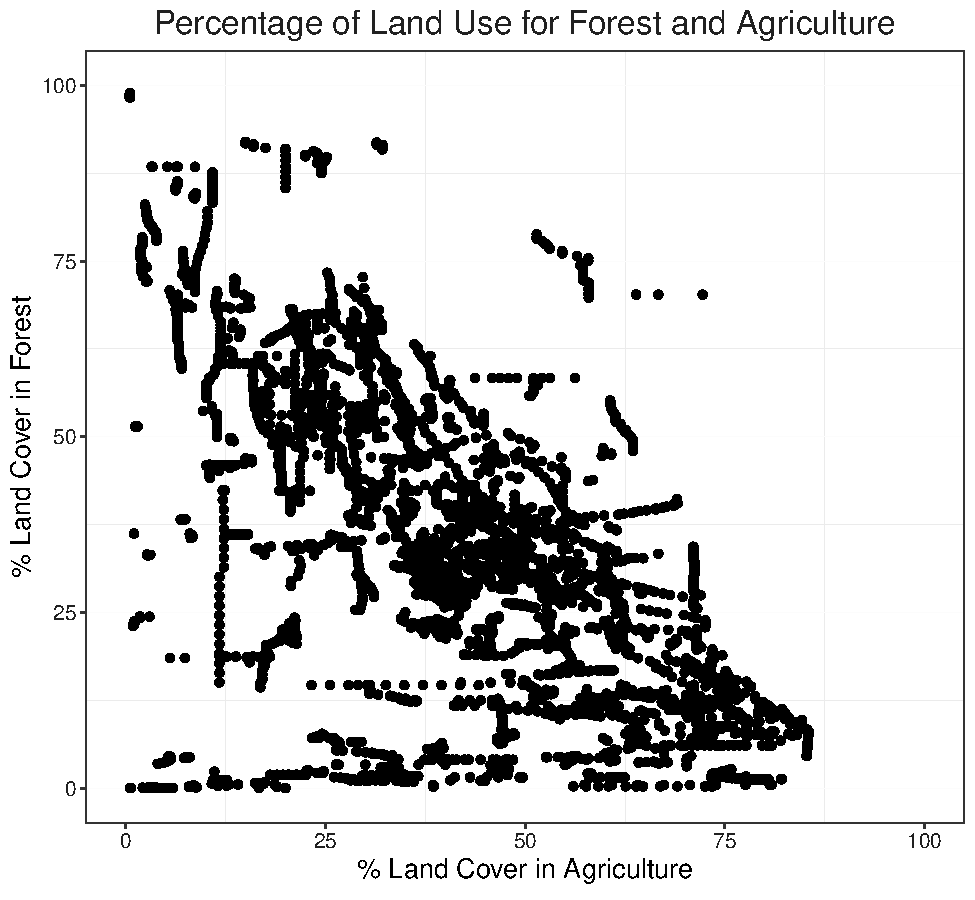
\includegraphics{Marx_ENV872_Project_files/figure-latex/fig1-1.pdf}
\caption{\label{fig:fig1}Percentage of Land Use for Forest and
Agriculture}
\end{figure}

\begin{figure}
\centering
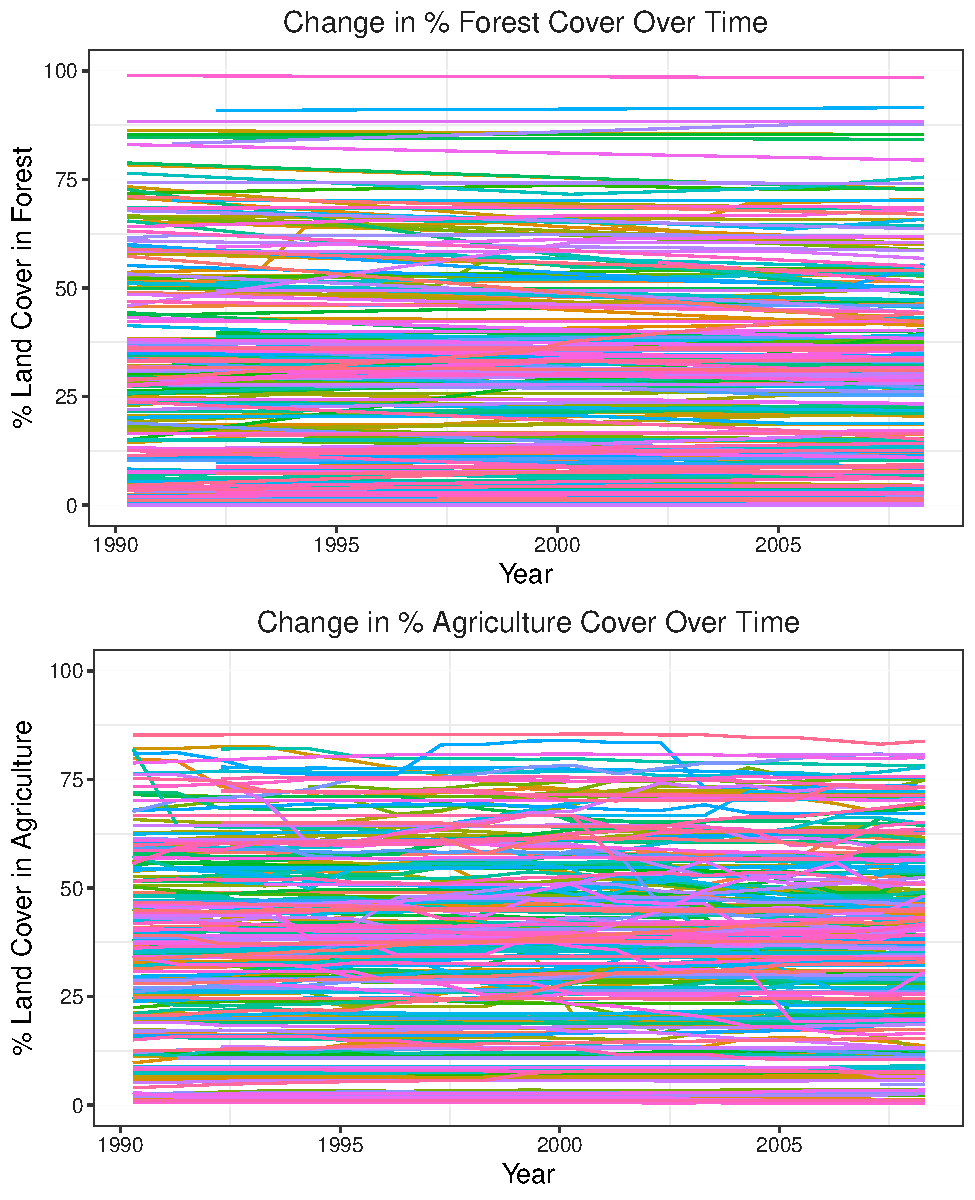
\includegraphics{Marx_ENV872_Project_files/figure-latex/unnamed-chunk-3-1.pdf}
\caption{\label{fig:fig2}Forest and Agriculture Cover Over Time}
\end{figure}

\begin{verbatim}
## `stat_bin()` using `bins = 30`. Pick better value with `binwidth`.
## `stat_bin()` using `bins = 30`. Pick better value with `binwidth`.
## `stat_bin()` using `bins = 30`. Pick better value with `binwidth`.
\end{verbatim}

\begin{figure}
\centering
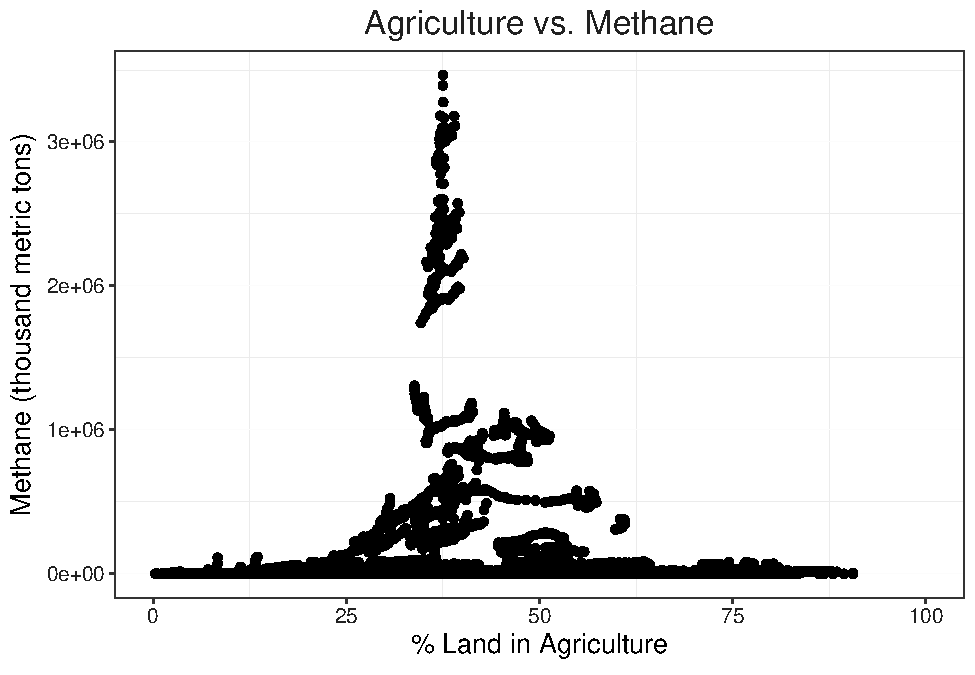
\includegraphics{Marx_ENV872_Project_files/figure-latex/unnamed-chunk-4-1.pdf}
\caption{\label{fig:fig3}Forest and Agriculture Data Distributions}
\end{figure}

\begin{verbatim}

\newpage
 
\end{verbatim}

\section{Analysis}\label{analysis}

\begin{verbatim}
##Forest Cover and Impacts of Agriculture
\end{verbatim}

Given that forest cover is my main variable of interest, I started by
testing of forest cover changes over time.

I used hierarchical or mixed-effect model to include the variable time,
expressed in years. I did not set up the model to deal with temporal
autocorrelation because, given that there was only one observation per
location per year, I did not believe there would be an issue with
seasonality.

I initially attempted three models: a generalized least squares model
fit by REML; a linear mixed-effects (LME) model fit by REML with
countries as a random effect, and a generalized linear squares (GLS)
model which did not allow me to account for fixed effects and random
effects. I attempted the GLS because my Forest and Agriculture variables
are both measured as percentages meaning a logit model might be more
appropriate. GLS allows for non-normal distributions. However, the
results of the GLS model were similar to the GLM model which allows for
random effects. Both appeared inferior to the LME model which had a
lower AIC of 49431 versus 49977 for GLS and 49967 for GLM. As such, I
used LME going forward.

The LME model revealed that forest does change over time with a negative
coefficient of -.00424 and a p-value of 0.00. It is difficult to
directly interpret this becasue the chosen model structure may not be
perfect, but this could be read: on average, there is .004\% decrease in
forest cover every year.

\begin{verbatim}
\end{verbatim}

\begin{Shaded}
\begin{Highlighting}[]
\CommentTok{#Statistical Test 1: How has forest changed over time }
\NormalTok{Forest.Time1 <-}\StringTok{ }\KeywordTok{gls}\NormalTok{(}\DataTypeTok{data =}\NormalTok{ WB_Spread, }
\NormalTok{                    Forest }\OperatorTok{~}\StringTok{ }\NormalTok{Year,}
                    \DataTypeTok{method =} \StringTok{"REML"}\NormalTok{)}
\KeywordTok{summary}\NormalTok{(Forest.Time1)}
\end{Highlighting}
\end{Shaded}

\begin{verbatim}
## Generalized least squares fit by REML
##   Model: Forest ~ Year 
##   Data: WB_Spread 
##        AIC      BIC    logLik
##   49977.96 49997.13 -24985.98
## 
## Coefficients:
##                Value Std.Error   t-value p-value
## (Intercept) 83.48572  5.840169 14.295086       0
## Year        -0.00425  0.000533 -7.987907       0
## 
##  Correlation: 
##      (Intr)
## Year -0.984
## 
## Standardized residuals:
##         Min          Q1         Med          Q3         Max 
## -0.74247841 -0.33743857 -0.09641382  0.15552883 16.46833243 
## 
## Residual standard error: 69.98862 
## Degrees of freedom: 4408 total; 4406 residual
\end{verbatim}

\begin{Shaded}
\begin{Highlighting}[]
\NormalTok{Forest.Time2 <-}\StringTok{ }\KeywordTok{lme}\NormalTok{(}\DataTypeTok{data =}\NormalTok{ WB_Spread,}
\NormalTok{                Forest }\OperatorTok{~}\StringTok{ }\NormalTok{Year,}
                \DataTypeTok{random =} \OperatorTok{~}\DecValTok{1}\OperatorTok{|}\StringTok{ }\NormalTok{Country,}
                \DataTypeTok{method =} \StringTok{"REML"}\NormalTok{)}
\KeywordTok{summary}\NormalTok{(Forest.Time2)}
\end{Highlighting}
\end{Shaded}

\begin{verbatim}
## Linear mixed-effects model fit by REML
##  Data: WB_Spread 
##        AIC      BIC    logLik
##   49431.95 49457.52 -24711.98
## 
## Random effects:
##  Formula: ~1 | Country
##         (Intercept) Residual
## StdDev:    30.52692 62.84915
## 
## Fixed effects: Forest ~ Year 
##                Value Std.Error   DF   t-value p-value
## (Intercept) 82.97070  5.654288 4163 14.673944       0
## Year        -0.00421  0.000482 4163 -8.743567       0
##  Correlation: 
##      (Intr)
## Year -0.923
## 
## Standardized Within-Group Residuals:
##         Min          Q1         Med          Q3         Max 
## -2.55113019 -0.14187377 -0.01873545  0.09332491 16.07509035 
## 
## Number of Observations: 4408
## Number of Groups: 244
\end{verbatim}

\begin{Shaded}
\begin{Highlighting}[]
\NormalTok{Logit_Test <-}\StringTok{ }\KeywordTok{glm}\NormalTok{(}\DataTypeTok{data =}\NormalTok{ WB_Spread,}
\NormalTok{             Forest }\OperatorTok{~}\StringTok{ }\NormalTok{Year)}
\KeywordTok{summary}\NormalTok{(Logit_Test)}
\end{Highlighting}
\end{Shaded}

\begin{verbatim}
## 
## Call:
## glm(formula = Forest ~ Year, data = WB_Spread)
## 
## Deviance Residuals: 
##     Min       1Q   Median       3Q      Max  
##  -51.97   -23.62    -6.75    10.89  1152.60  
## 
## Coefficients:
##               Estimate Std. Error t value Pr(>|t|)    
## (Intercept) 83.4857163  5.8401690  14.295  < 2e-16 ***
## Year        -0.0042538  0.0005325  -7.988 1.74e-15 ***
## ---
## Signif. codes:  0 '***' 0.001 '**' 0.01 '*' 0.05 '.' 0.1 ' ' 1
## 
## (Dispersion parameter for gaussian family taken to be 4898.407)
## 
##     Null deviance: 21894930  on 4407  degrees of freedom
## Residual deviance: 21582379  on 4406  degrees of freedom
## AIC: 49967
## 
## Number of Fisher Scoring iterations: 2
\end{verbatim}

After establishing that there is a change in forest cover over time, I
ran an LME regression to see if agriculture cover can explain any of the
change in forest cover. The result of the test was a statistically
significant (p-value = 0.00) negative relationship which, in absolute
terms, can be interpreted as a 1\% increase in agriculture cover results
in a .49\% decrease in forest cover.

I used a test for correlation to better understand this relationship. It
revealed that there is slight negative correlation between agriculture
and forest with a 95\% confidence interval of -.16 and -.10. ```

\begin{Shaded}
\begin{Highlighting}[]
\NormalTok{For.Ag.}\DecValTok{2}\NormalTok{ <-}\StringTok{  }\KeywordTok{lme}\NormalTok{(}\DataTypeTok{data =}\NormalTok{ WB_Spread,}
\NormalTok{              Forest }\OperatorTok{~}\StringTok{ }\NormalTok{Year }\OperatorTok{+}\StringTok{ }\NormalTok{Agriculture,}
              \DataTypeTok{random =} \OperatorTok{~}\DecValTok{1}\OperatorTok{|}\StringTok{ }\NormalTok{Country,}
              \DataTypeTok{method =} \StringTok{"REML"}\NormalTok{)}
\KeywordTok{summary}\NormalTok{(For.Ag.}\DecValTok{2}\NormalTok{)}
\end{Highlighting}
\end{Shaded}

\begin{verbatim}
## Linear mixed-effects model fit by REML
##  Data: WB_Spread 
##       AIC      BIC    logLik
##   49413.7 49445.65 -24701.85
## 
## Random effects:
##  Formula: ~1 | Country
##         (Intercept) Residual
## StdDev:    29.32764 62.80075
## 
## Fixed effects: Forest ~ Year + Agriculture 
##                 Value Std.Error   DF   t-value p-value
## (Intercept) 101.79318  6.830657 4162 14.902399       0
## Year         -0.00421  0.000481 4162 -8.754338       0
## Agriculture  -0.49055  0.101138 4162 -4.850333       0
##  Correlation: 
##             (Intr) Year  
## Year        -0.763       
## Agriculture -0.568  0.000
## 
## Standardized Within-Group Residuals:
##         Min          Q1         Med          Q3         Max 
## -2.53066671 -0.13903414 -0.01968184  0.09295492 16.10850732 
## 
## Number of Observations: 4408
## Number of Groups: 244
\end{verbatim}

\begin{Shaded}
\begin{Highlighting}[]
\KeywordTok{cor.test}\NormalTok{(}\DataTypeTok{formula =} \OperatorTok{~}\StringTok{ }\NormalTok{Forest }\OperatorTok{+}\StringTok{ }\NormalTok{Agriculture,}
         \DataTypeTok{data =}\NormalTok{ WB_Spread)}
\end{Highlighting}
\end{Shaded}

\begin{verbatim}
## 
##  Pearson's product-moment correlation
## 
## data:  Forest and Agriculture
## t = -8.7073, df = 4406, p-value < 2.2e-16
## alternative hypothesis: true correlation is not equal to 0
## 95 percent confidence interval:
##  -0.1589757 -0.1009293
## sample estimates:
##        cor 
## -0.1300639
\end{verbatim}

To visualize the relationship between agriculture and forest, I chose to
display one country from each of 5 major continents: North America,
South America, Europe, Asia and Africa in
\textbf{(Figure\ref{fig:fig4})}. The country selection within regions
was semi-random. I anticipated that Brazil and Indonesia might show
increasing agriculture with decreasing forest based on past research;
Canada, Spain and Kenya were chosen at random with the understanding
that these five countries represent different regions and states of
economic development. The graph shows that forest and agriculture, when
they do move, do indeed tend to have an inverse relationship.
Agriculture is not always leading to a decrease in forest cover, but
three of the five samples are moving in oposite directions while the
other two have fairly constant levels.

\begin{figure}
\centering
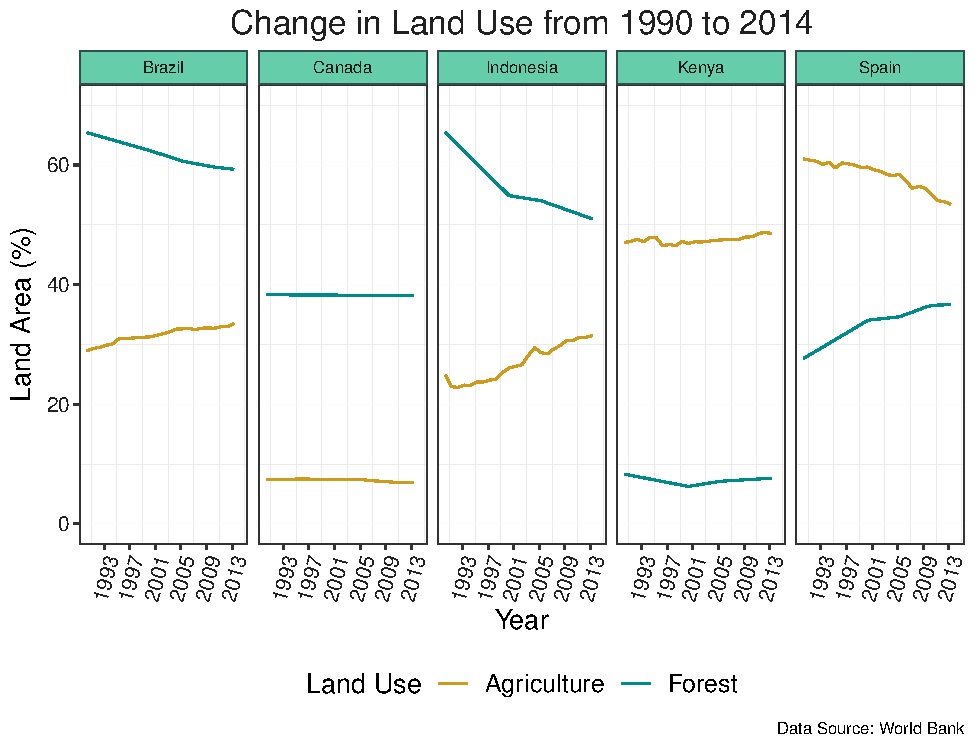
\includegraphics{Marx_ENV872_Project_files/figure-latex/unnamed-chunk-7-1.pdf}
\caption{\label{fig:fig4}Change in Land Use from 1990 to 2014 for Five
Countries}
\end{figure}

\subsection{Spotlight on Brazil}\label{spotlight-on-brazil}

Zooming in more narrowly on one country, I used Pettit's test, a
nonparametric test that determines if there is a shift in the central
tendency of the time series, to determine at what point in time the
changepoints occur in Brazil. I applied the test to both Forest Cover
and Agriculture Cover to 1) see if there was a change point for
agriculture and/or forest and 2) see if the change points occured in the
same year for both forest and agriculture.

Pettitt's applied to a single country (Brazil) initially detects a
change point in Forest and Agriculture in the same year. The change for
both was in place 13, which is the year 2002 with a p-value of .0001 in
both instances. The second change points were only a year apart, as seen
in \textbf{(Figure\ref{fig:fig5})}. This is an exmaple of agriculture
and forest covers moving inversely at the same time. In the case of
Spain, the first detected change points occured two years apart. In
Kenya, the first detected change points for forest and agricuture covers
were 8 years apart.

\begin{Shaded}
\begin{Highlighting}[]
\CommentTok{#Statistical Test 2: Pettitts Test: Looking at Change Points in the Data}

\CommentTok{#Statistical Test 2: Any change points for full forest data?}
\KeywordTok{pettitt.test}\NormalTok{(WB_Spread}\OperatorTok{$}\NormalTok{Forest)}
\end{Highlighting}
\end{Shaded}

\begin{verbatim}
## 
##  Pettitt's test for single change-point detection
## 
## data:  WB_Spread$Forest
## U* = 463360, p-value = 5.895e-07
## alternative hypothesis: two.sided
## sample estimates:
## probable change point at time K 
##                            1739
\end{verbatim}

\begin{Shaded}
\begin{Highlighting}[]
\CommentTok{#Probable change point at time 1428 which doesn't exist.}

\NormalTok{WB_Brazil <-}\StringTok{ }\KeywordTok{select}\NormalTok{(WB_Brazil, Forest, Agriculture, Country, Year) }\OperatorTok
\StringTok{  }\NormalTok{na.exclude}

\CommentTok{#Changes in Brazil Forest}
\KeywordTok{pettitt.test}\NormalTok{(WB_Brazil}\OperatorTok{$}\NormalTok{Forest)}
\end{Highlighting}
\end{Shaded}

\begin{verbatim}
## 
##  Pettitt's test for single change-point detection
## 
## data:  WB_Brazil$Forest
## U* = 182, p-value = 0.0001182
## alternative hypothesis: two.sided
## sample estimates:
## probable change point at time K                            <NA> 
##                              13                              14
\end{verbatim}

\begin{Shaded}
\begin{Highlighting}[]
\KeywordTok{pettitt.test}\NormalTok{(WB_Brazil}\OperatorTok{$}\NormalTok{Forest[}\DecValTok{13}\OperatorTok{:}\DecValTok{27}\NormalTok{])}
\end{Highlighting}
\end{Shaded}

\begin{verbatim}
## 
##  Pettitt's test for single change-point detection
## 
## data:  WB_Brazil$Forest[13:27]
## U* = 56, p-value = 0.01074
## alternative hypothesis: two.sided
## sample estimates:
## probable change point at time K                            <NA> 
##                               7                               8
\end{verbatim}

\begin{Shaded}
\begin{Highlighting}[]
\KeywordTok{pettitt.test}\NormalTok{(WB_Brazil}\OperatorTok{$}\NormalTok{Forest[}\DecValTok{20}\OperatorTok{:}\DecValTok{27}\NormalTok{])}
\end{Highlighting}
\end{Shaded}

\begin{verbatim}
## 
##  Pettitt's test for single change-point detection
## 
## data:  WB_Brazil$Forest[20:27]
## U* = 16, p-value = 0.139
## alternative hypothesis: two.sided
## sample estimates:
## probable change point at time K 
##                               4
\end{verbatim}

\begin{Shaded}
\begin{Highlighting}[]
\CommentTok{#Changes in Brazil Agriculture }

\KeywordTok{pettitt.test}\NormalTok{(WB_Brazil}\OperatorTok{$}\NormalTok{Agriculture)}
\end{Highlighting}
\end{Shaded}

\begin{verbatim}
## 
##  Pettitt's test for single change-point detection
## 
## data:  WB_Brazil$Agriculture
## U* = 182, p-value = 0.0001182
## alternative hypothesis: two.sided
## sample estimates:
## probable change point at time K                            <NA> 
##                              13                              14
\end{verbatim}

\begin{Shaded}
\begin{Highlighting}[]
\KeywordTok{pettitt.test}\NormalTok{(WB_Brazil}\OperatorTok{$}\NormalTok{Agriculture[}\DecValTok{13}\OperatorTok{:}\DecValTok{27}\NormalTok{])}
\end{Highlighting}
\end{Shaded}

\begin{verbatim}
## 
##  Pettitt's test for single change-point detection
## 
## data:  WB_Brazil$Agriculture[13:27]
## U* = 54, p-value = 0.0155
## alternative hypothesis: two.sided
## sample estimates:
## probable change point at time K                            <NA> 
##                               6                               7 
##                            <NA> 
##                               9
\end{verbatim}

\begin{Shaded}
\begin{Highlighting}[]
\KeywordTok{pettitt.test}\NormalTok{(WB_Brazil}\OperatorTok{$}\NormalTok{Agriculture[}\DecValTok{19}\OperatorTok{:}\DecValTok{27}\NormalTok{])}
\end{Highlighting}
\end{Shaded}

\begin{verbatim}
## 
##  Pettitt's test for single change-point detection
## 
## data:  WB_Brazil$Agriculture[19:27]
## U* = 20, p-value = 0.1033
## alternative hypothesis: two.sided
## sample estimates:
## probable change point at time K                            <NA> 
##                               4                               5
\end{verbatim}

\begin{Shaded}
\begin{Highlighting}[]
\CommentTok{#Spain}
\NormalTok{Spain.Pettit <-}\StringTok{ }\KeywordTok{filter}\NormalTok{(WB_Spread, Country }\OperatorTok{==}\StringTok{ "Spain"}\NormalTok{)}
\KeywordTok{pettitt.test}\NormalTok{(Spain.Pettit}\OperatorTok{$}\NormalTok{Forest)}
\end{Highlighting}
\end{Shaded}

\begin{verbatim}
## 
##  Pettitt's test for single change-point detection
## 
## data:  Spain.Pettit$Forest
## U* = 90, p-value = 0.002386
## alternative hypothesis: two.sided
## sample estimates:
## probable change point at time K                            <NA> 
##                               9                              10
\end{verbatim}

\begin{Shaded}
\begin{Highlighting}[]
\KeywordTok{pettitt.test}\NormalTok{(Spain.Pettit}\OperatorTok{$}\NormalTok{Agriculture)}
\end{Highlighting}
\end{Shaded}

\begin{verbatim}
## 
##  Pettitt's test for single change-point detection
## 
## data:  Spain.Pettit$Agriculture
## U* = 88, p-value = 0.003207
## alternative hypothesis: two.sided
## sample estimates:
## probable change point at time K 
##                              11
\end{verbatim}

\begin{Shaded}
\begin{Highlighting}[]
\CommentTok{#Kenya}
\NormalTok{Kenya.Pettit <-}\StringTok{ }\KeywordTok{filter}\NormalTok{(WB_Spread, Country }\OperatorTok{==}\StringTok{ "Kenya"}\NormalTok{)}
\KeywordTok{pettitt.test}\NormalTok{(Kenya.Pettit}\OperatorTok{$}\NormalTok{Forest)}
\end{Highlighting}
\end{Shaded}

\begin{verbatim}
## 
##  Pettitt's test for single change-point detection
## 
## data:  Kenya.Pettit$Forest
## U* = 76, p-value = 0.01646
## alternative hypothesis: two.sided
## sample estimates:
## probable change point at time K 
##                               6
\end{verbatim}

\begin{Shaded}
\begin{Highlighting}[]
\KeywordTok{pettitt.test}\NormalTok{(Kenya.Pettit}\OperatorTok{$}\NormalTok{Agriculture)}
\end{Highlighting}
\end{Shaded}

\begin{verbatim}
## 
##  Pettitt's test for single change-point detection
## 
## data:  Kenya.Pettit$Agriculture
## U* = 42, p-value = 0.4617
## alternative hypothesis: two.sided
## sample estimates:
## probable change point at time K 
##                              14
\end{verbatim}

\begin{figure}
\centering
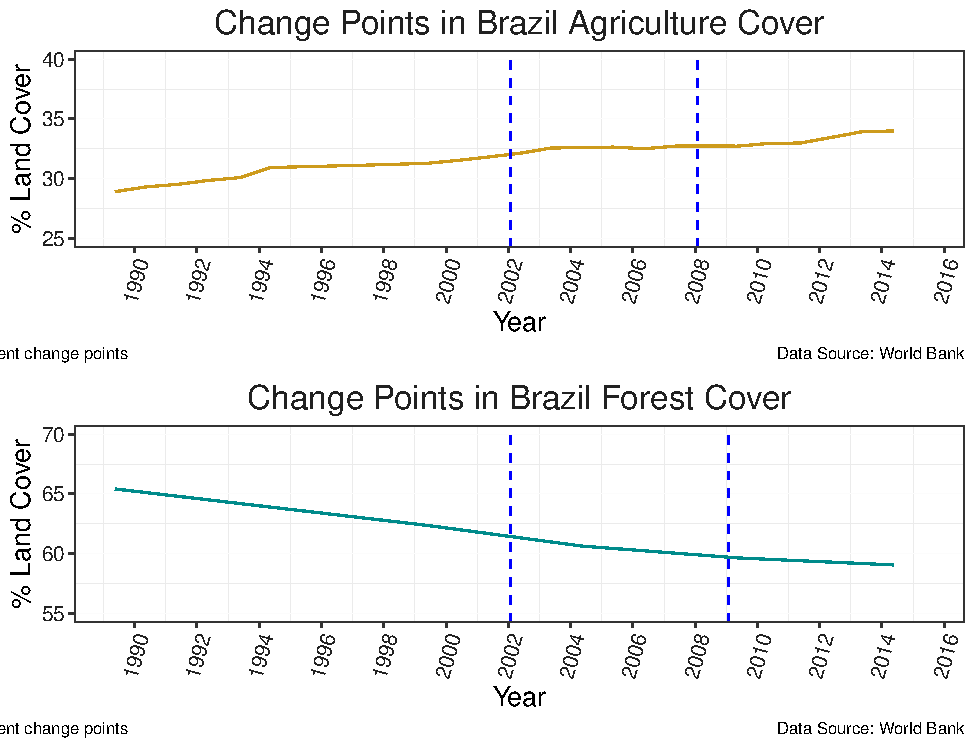
\includegraphics{Marx_ENV872_Project_files/figure-latex/unnamed-chunk-9-1.pdf}
\caption{\label{fig:fig5}Change Points in Brazil}
\end{figure}

\subsection{Evaluation of Electricity Variables as a Cause of
Deforestation}\label{evaluation-of-electricity-variables-as-a-cause-of-deforestation}

Having established that agriculture cover has an impact on forest cover,
I was also interested in whether access to electricity or the levels of
renewable energy produced in countries have a relationship with
deforestation. This is because a lack of electricity could drive the use
of forest biomass products as an energy source. To the contrary, when
included in a model with agriculture electricity access appears to have
a negative impact on forest (-.33 coefficient, p-value 0.00). This may
be because electricity is needed for some agricultural operations. To
test the idea that more agriculture may require more electricity, I ran
a variance inflation factor (vif) test to check for multicollinearity in
the model. The variance inflation factors were all around 1, meaning
multicollinearity is not a problem in the model. I also checked for
correlation using the cor.test which revealed that slightly negative
correlation between agriculture and electricity access, which I am
unable to explain.

A second theory regarding the negative relationship between electricity
access and forest cover is that electricity is produced via biofuels,
the production of which might require more forest to be converted to
agricultural land. With that theory in mind, I was interested in whether
there might be a relationship between forested land and renewable energy
output because energy produced from biomass is considered to be
renewable. However, the result of my LME revealed that a 1 unit increase
in renewable energy output is associated with an .20\% increase in
forest land, meaning the production of biofuels is likely not a main
driver of deforestation across the sample, or biofuel is a very small
portion of renewable energy.

These relationships can be observed in \textbf{(Figure\ref{fig:fig6})}
higlighting the chosen 5 countries.

\begin{Shaded}
\begin{Highlighting}[]
\CommentTok{#Looking at Electricity Accesss and Renewable Energy }
\CommentTok{#as a Driver of the Ag. / Forest Tradeoff}

\NormalTok{Forest.Ag.Elec <-}\StringTok{ }\KeywordTok{lme}\NormalTok{(}\DataTypeTok{data =}\NormalTok{ WB_Spread, }
\NormalTok{                    Forest }\OperatorTok{~}\StringTok{ }\NormalTok{Year }\OperatorTok{+}\StringTok{ }\NormalTok{Agriculture }\OperatorTok{+}\StringTok{ }\NormalTok{ElectricityAccess,}
                    \DataTypeTok{random =} \OperatorTok{~}\DecValTok{1}\OperatorTok{|}\StringTok{ }\NormalTok{Country,}
                    \DataTypeTok{method =} \StringTok{"REML"}\NormalTok{)}
\KeywordTok{summary}\NormalTok{(Forest.Ag.Elec)}
\end{Highlighting}
\end{Shaded}

\begin{verbatim}
## Linear mixed-effects model fit by REML
##  Data: WB_Spread 
##       AIC      BIC   logLik
##   49390.4 49428.74 -24689.2
## 
## Random effects:
##  Formula: ~1 | Country
##         (Intercept) Residual
## StdDev:    27.83298 62.73873
## 
## Fixed effects: Forest ~ Year + Agriculture + ElectricityAccess 
##                       Value Std.Error   DF   t-value p-value
## (Intercept)       120.57059  7.551404 4161 15.966644       0
## Year               -0.00360  0.000494 4161 -7.293828       0
## Agriculture        -0.54735  0.097884 4161 -5.591834       0
## ElectricityAccess  -0.32406  0.059178 4161 -5.475929       0
##  Correlation: 
##                   (Intr) Year   Agrclt
## Year              -0.567              
## Agriculture       -0.542 -0.026       
## ElectricityAccess -0.458 -0.227  0.113
## 
## Standardized Within-Group Residuals:
##         Min          Q1         Med          Q3         Max 
## -2.55910898 -0.13847664 -0.01628249  0.09483862 16.10165562 
## 
## Number of Observations: 4408
## Number of Groups: 244
\end{verbatim}

\begin{Shaded}
\begin{Highlighting}[]
\NormalTok{car}\OperatorTok{::}\KeywordTok{vif}\NormalTok{(Forest.Ag.Elec)}
\end{Highlighting}
\end{Shaded}

\begin{verbatim}
##              Year       Agriculture ElectricityAccess 
##          1.054359          1.013011          1.067362
\end{verbatim}

\begin{Shaded}
\begin{Highlighting}[]
\KeywordTok{cor.test}\NormalTok{(}\DataTypeTok{formula =} \OperatorTok{~}\StringTok{ }\NormalTok{ElectricityAccess }\OperatorTok{+}\StringTok{ }\NormalTok{Agriculture,}
         \DataTypeTok{data =}\NormalTok{ WB_Spread)}
\end{Highlighting}
\end{Shaded}

\begin{verbatim}
## 
##  Pearson's product-moment correlation
## 
## data:  ElectricityAccess and Agriculture
## t = -9.0997, df = 4406, p-value < 2.2e-16
## alternative hypothesis: true correlation is not equal to 0
## 95 percent confidence interval:
##  -0.1646811 -0.1067250
## sample estimates:
##        cor 
## -0.1358192
\end{verbatim}

\begin{Shaded}
\begin{Highlighting}[]
\NormalTok{Forest.RE <-}\StringTok{ }\KeywordTok{lme}\NormalTok{(}\DataTypeTok{data =}\NormalTok{ WB_Spread, }
\NormalTok{                    Forest }\OperatorTok{~}\StringTok{ }\NormalTok{Year }\OperatorTok{+}\StringTok{ }\NormalTok{RenewableElectricity,}
                    \DataTypeTok{random =} \OperatorTok{~}\DecValTok{1} \OperatorTok{|}\StringTok{ }\NormalTok{Country,}
                    \DataTypeTok{method =} \StringTok{"REML"}\NormalTok{)}
\KeywordTok{summary}\NormalTok{(Forest.RE)}
\end{Highlighting}
\end{Shaded}

\begin{verbatim}
## Linear mixed-effects model fit by REML
##  Data: WB_Spread 
##        AIC      BIC    logLik
##   49426.51 49458.46 -24708.26
## 
## Random effects:
##  Formula: ~1 | Country
##         (Intercept) Residual
## StdDev:    29.95973  62.8271
## 
## Fixed effects: Forest ~ Year + RenewableElectricity 
##                         Value Std.Error   DF   t-value p-value
## (Intercept)          75.74745  6.033345 4162 12.554801   0e+00
## Year                 -0.00411  0.000482 4162 -8.520768   0e+00
## RenewableElectricity  0.20104  0.059653 4162  3.370074   8e-04
##  Correlation: 
##                      (Intr) Year  
## Year                 -0.885       
## RenewableElectricity -0.355  0.062
## 
## Standardized Within-Group Residuals:
##         Min          Q1         Med          Q3         Max 
## -2.56121812 -0.14368890 -0.02045123  0.09519242 16.07197971 
## 
## Number of Observations: 4408
## Number of Groups: 244
\end{verbatim}

\begin{figure}
\centering
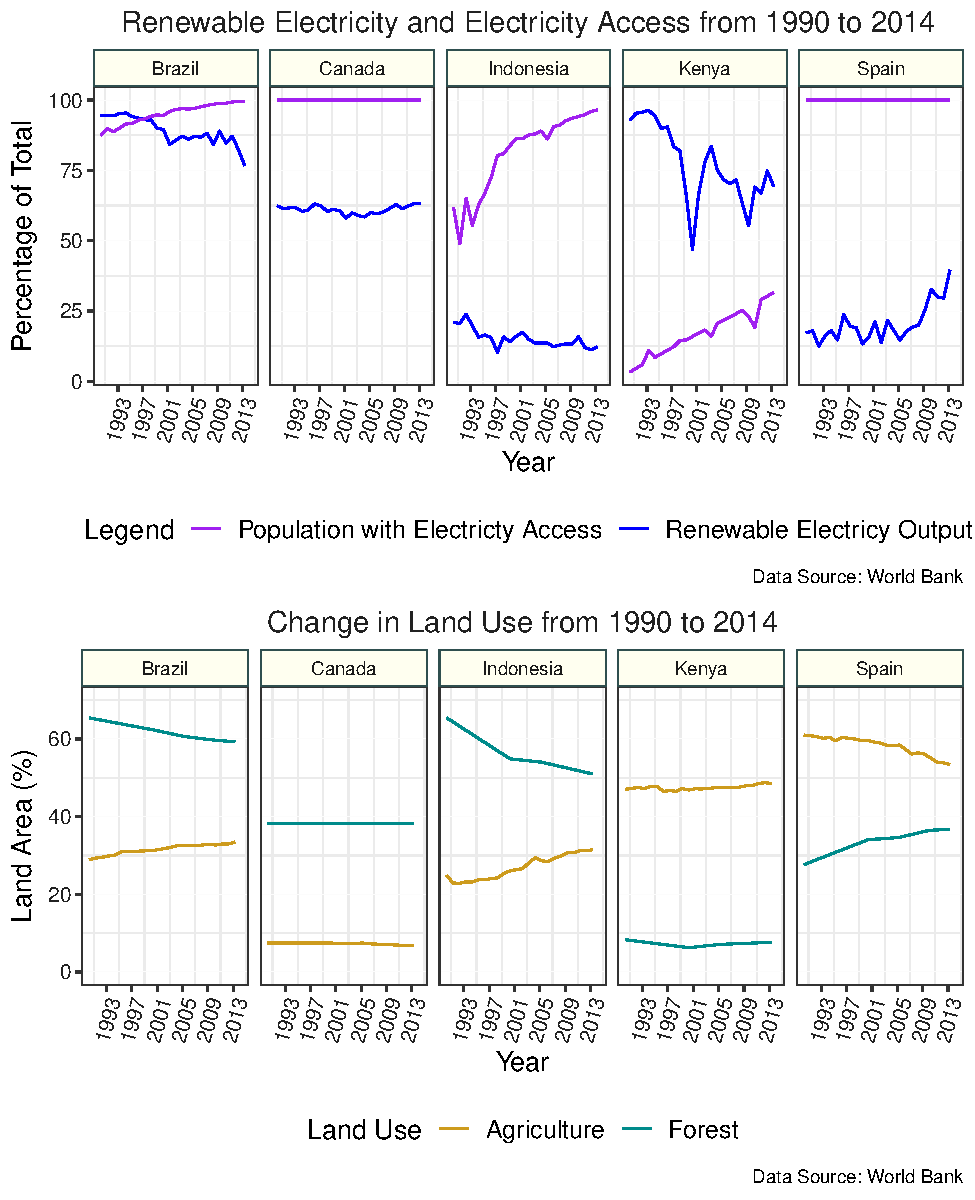
\includegraphics{Marx_ENV872_Project_files/figure-latex/unnamed-chunk-11-1.pdf}
\caption{\label{fig:fig6}Electricity Trends for Five Countries}
\end{figure}

\subsection{A Look at Emissions}\label{a-look-at-emissions}

The next series of tests address the question: Is there a relationship
between land uses (agriculture or forest) and levels of CO2, methane,
and NO3 emissions?

In a model with methane as the dependent variable and forest and
agriculture as the explanatory variables, A 1\% increase in agriculture
leads to an increase of methane of 662.28 thousand metric tons of CO2
equivalent (p-value 0.00); A 1\% increase in forest leads to a decrease
of methane of -17.51 thousand metric tons of CO2 equivalent (p-value
.003). I have tested this model for multicollinearity given the
significant relationship between agriculture and forest, but it does not
seem to be a problem in this model with VIFs around 1. The coefficients
are only slightly different that if I made two separate models for
agriculture and forest.

In a model with N2O as the dependent variable and forest and agriculture
as the explanatory variables, A 1\% increase in agriculture leads to an
increase of nitrous oxide (N2O) of 491.079 thousand metric tons of CO2
equivalent (p-value 0.002); A 1\% increase in forest leads to a decrease
of nitrous oxide of -1.526 thousand metric tons of CO2 equivalent, but
this is not statistically significant with a p-value of .7986.

The results for carbon emissions were not statistically significant,
likely because the number includes a large percentage of carbon
emissions that are associated with the manufacturing sector as opposed
to carbon from land use changes.

All of these emissions changes over time can be compared to forest and
agriculture cover changes for five countries in
\textbf{(Figure\ref{fig:fig7})}.

\begin{Shaded}
\begin{Highlighting}[]
\CommentTok{#Methane Emissions}
\NormalTok{Ag.For.Meth <-}\StringTok{ }\KeywordTok{lme}\NormalTok{(}\DataTypeTok{data =}\NormalTok{ WB_Spread,}
\NormalTok{                 Ag.Methane }\OperatorTok{~}\StringTok{ }\NormalTok{Year }\OperatorTok{+}\StringTok{ }\NormalTok{Agriculture }\OperatorTok{+}\StringTok{ }\NormalTok{Forest,}
                 \DataTypeTok{random =} \OperatorTok{~}\DecValTok{1}\OperatorTok{|}\StringTok{ }\NormalTok{Country,}
                 \DataTypeTok{method =} \StringTok{"REML"}\NormalTok{)}
\KeywordTok{summary}\NormalTok{(Ag.For.Meth)}
\end{Highlighting}
\end{Shaded}

\begin{verbatim}
## Linear mixed-effects model fit by REML
##  Data: WB_Spread 
##        AIC      BIC    logLik
##   103404.4 103442.8 -51696.22
## 
## Random effects:
##  Formula: ~1 | Country
##         (Intercept) Residual
## StdDev:    399120.3 23820.09
## 
## Fixed effects: Ag.Methane ~ Year + Agriculture + Forest 
##                Value Std.Error   DF   t-value p-value
## (Intercept) 87511.28 26372.723 4161  3.318250  0.0009
## Year            1.93     0.185 4161 10.410309  0.0000
## Agriculture   662.28   160.104 4161  4.136567  0.0000
## Forest        -17.51     5.879 4161 -2.978478  0.0029
##  Correlation: 
##             (Intr) Year   Agrclt
## Year        -0.082              
## Agriculture -0.235  0.021       
## Forest      -0.031  0.134  0.052
## 
## Standardized Within-Group Residuals:
##         Min          Q1         Med          Q3         Max 
## -5.12554859 -0.17369030 -0.02167479  0.13084901 14.13409745 
## 
## Number of Observations: 4408
## Number of Groups: 244
\end{verbatim}

\begin{Shaded}
\begin{Highlighting}[]
\NormalTok{car}\OperatorTok{::}\KeywordTok{vif}\NormalTok{(Ag.For.Meth)}
\end{Highlighting}
\end{Shaded}

\begin{verbatim}
##        Year Agriculture      Forest 
##    1.018527    1.002885    1.020821
\end{verbatim}

\begin{Shaded}
\begin{Highlighting}[]
\CommentTok{#NO2 Emissions}
\NormalTok{Ag.For.N2O <-}\StringTok{ }\KeywordTok{lme}\NormalTok{(}\DataTypeTok{data =}\NormalTok{ WB_Spread,}
\NormalTok{                 Ag.N2O }\OperatorTok{~}\StringTok{ }\NormalTok{Year }\OperatorTok{+}\StringTok{ }\NormalTok{Agriculture }\OperatorTok{+}\StringTok{ }\NormalTok{Forest,}
                 \DataTypeTok{random =} \OperatorTok{~}\DecValTok{1}\OperatorTok{|}\StringTok{ }\NormalTok{Country,}
                 \DataTypeTok{method =} \StringTok{"REML"}\NormalTok{)}
\KeywordTok{summary}\NormalTok{(Ag.For.N2O)}
\end{Highlighting}
\end{Shaded}

\begin{verbatim}
## Linear mixed-effects model fit by REML
##  Data: WB_Spread 
##        AIC      BIC    logLik
##   103271.9 103310.3 -51629.97
## 
## Random effects:
##  Formula: ~1 | Country
##         (Intercept) Residual
## StdDev:    227178.8 24227.78
## 
## Fixed effects: Ag.N2O ~ Year + Agriculture + Forest 
##                 Value Std.Error   DF   t-value p-value
## (Intercept) 27911.574 15946.871 4161  1.750285  0.0801
## Year            2.963     0.188 4161 15.742913  0.0000
## Agriculture   491.079   160.038 4161  3.068527  0.0022
## Forest         -1.526     5.980 4161 -0.255123  0.7986
##  Correlation: 
##             (Intr) Year   Agrclt
## Year        -0.138              
## Agriculture -0.388  0.021       
## Forest      -0.051  0.134  0.051
## 
## Standardized Within-Group Residuals:
##        Min         Q1        Med         Q3        Max 
## -6.2159495 -0.2384565 -0.0193730  0.1994855 15.2698912 
## 
## Number of Observations: 4408
## Number of Groups: 244
\end{verbatim}

\begin{Shaded}
\begin{Highlighting}[]
\NormalTok{car}\OperatorTok{::}\KeywordTok{vif}\NormalTok{(Ag.For.N2O)}
\end{Highlighting}
\end{Shaded}

\begin{verbatim}
##        Year Agriculture      Forest 
##    1.018512    1.002841    1.020782
\end{verbatim}

\begin{Shaded}
\begin{Highlighting}[]
\CommentTok{#CO2 Emissions}
\NormalTok{Ag.For.CO2 <-}\StringTok{ }\KeywordTok{lme}\NormalTok{(}\DataTypeTok{data =}\NormalTok{ WB_Spread,}
\NormalTok{                 CO2Emissions }\OperatorTok{~}\StringTok{ }\NormalTok{Year }\OperatorTok{+}\StringTok{ }\NormalTok{Agriculture }\OperatorTok{+}\StringTok{ }\NormalTok{Forest,}
                 \DataTypeTok{random =} \OperatorTok{~}\DecValTok{1}\OperatorTok{|}\StringTok{ }\NormalTok{Country,}
                 \DataTypeTok{method =} \StringTok{"REML"}\NormalTok{)}
\KeywordTok{summary}\NormalTok{(Ag.For.CO2)}
\end{Highlighting}
\end{Shaded}

\begin{verbatim}
## Linear mixed-effects model fit by REML
##  Data: WB_Spread 
##        AIC      BIC   logLik
##   129304.6 129342.9 -64646.3
## 
## Random effects:
##  Formula: ~1 | Country
##         (Intercept) Residual
## StdDev:     2815249 477534.2
## 
## Fixed effects: CO2Emissions ~ Year + Agriculture + Forest 
##                 Value Std.Error   DF   t-value p-value
## (Intercept) 237143.25 219216.50 4161  1.081776  0.2794
## Year            62.69      3.71 4161 16.899691  0.0000
## Agriculture   -972.29   3040.95 4161 -0.319733  0.7492
## Forest         -67.45    117.84 4161 -0.572366  0.5671
##  Correlation: 
##             (Intr) Year   Agrclt
## Year        -0.197              
## Agriculture -0.536  0.020       
## Forest      -0.072  0.134  0.051
## 
## Standardized Within-Group Residuals:
##          Min           Q1          Med           Q3          Max 
## -6.645266358 -0.228318747 -0.009787546  0.194387104 13.617669525 
## 
## Number of Observations: 4408
## Number of Groups: 244
\end{verbatim}

\begin{Shaded}
\begin{Highlighting}[]
\NormalTok{ForCO2 <-}\StringTok{ }\KeywordTok{lme}\NormalTok{(}\DataTypeTok{data =}\NormalTok{ WB_Spread,}
\NormalTok{                 Ag.Methane }\OperatorTok{~}\StringTok{ }\NormalTok{Year }\OperatorTok{+}\StringTok{ }\NormalTok{Forest,}
                 \DataTypeTok{random =} \OperatorTok{~}\DecValTok{1}\OperatorTok{|}\StringTok{ }\NormalTok{Country,}
                 \DataTypeTok{method =} \StringTok{"REML"}\NormalTok{)}
\KeywordTok{summary}\NormalTok{(ForCO2)}
\end{Highlighting}
\end{Shaded}

\begin{verbatim}
## Linear mixed-effects model fit by REML
##  Data: WB_Spread 
##        AIC      BIC    logLik
##   103431.5 103463.5 -51710.76
## 
## Random effects:
##  Formula: ~1 | Country
##         (Intercept) Residual
## StdDev:    399211.3 23865.83
## 
## Fixed effects: Ag.Methane ~ Year + Forest 
##                 Value Std.Error   DF   t-value p-value
## (Intercept) 113115.75 25642.184 4162  4.411315  0.0000
## Year             1.91     0.185 4162 10.306589  0.0000
## Forest         -18.77     5.883 4162 -3.190742  0.0014
##  Correlation: 
##        (Intr) Year  
## Year   -0.080       
## Forest -0.019  0.133
## 
## Standardized Within-Group Residuals:
##         Min          Q1         Med          Q3         Max 
## -5.11273090 -0.17479056 -0.02340015  0.13160047 14.10832094 
## 
## Number of Observations: 4408
## Number of Groups: 244
\end{verbatim}

\begin{figure}
\centering
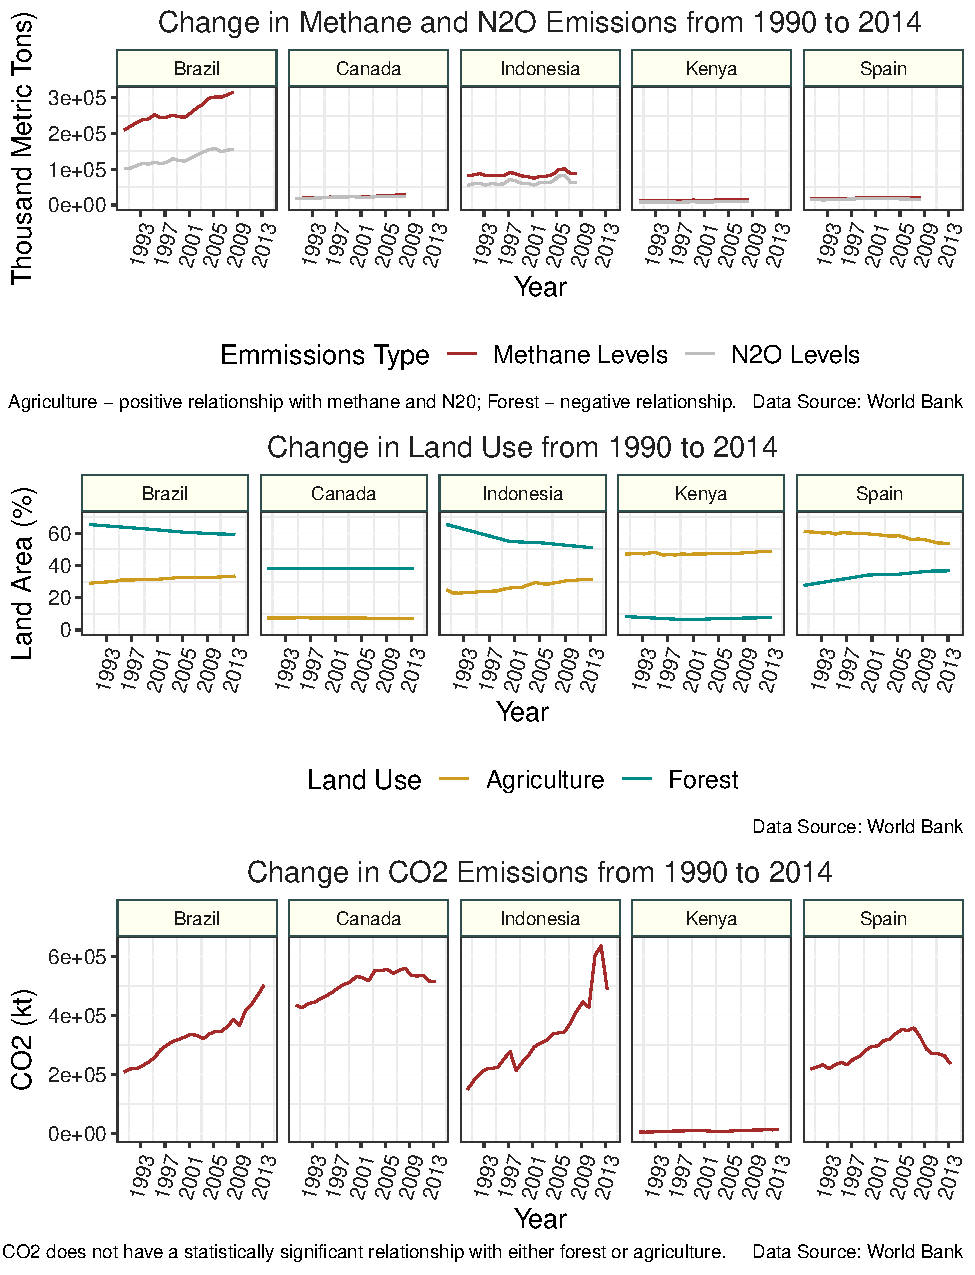
\includegraphics{Marx_ENV872_Project_files/figure-latex/unnamed-chunk-13-1.pdf}
\caption{\label{fig:fig7}Change in Emissions Use from 1990 to 2014 for
Five Countries}
\end{figure}

\begin{verbatim}


\end{verbatim}

\begin{verbatim}

\end{verbatim}

\newpage

\section{Summary and Conclusions}\label{summary-and-conclusions}

\subsection{Summary}\label{summary}

This research has looks at the causes and impacts of changes in land use
from 1990 to 2014 as it pertains to forest cover and agriculture cover.
There is a statistically significant trend of slightly decreasing forest
cover over time in the full data set of 263 countries, which can
partially be attributed to changes in agriculture cover. Renewable
electricity output and electricity access also have statistically
significant relationships with forest cover. Meanwhile, on the other end
of the spectrum, changes in land dedicated to agriculture and to forest
have explained increases in emissions of agricultural methane and
nitrous oxide, though they were not able to explain changes in CO2.

The questions this research attempts to answer are addressed below:

\textbf{Is there a relationship between the percentage of land area
dedicated to forest versus agricultural in countries?}

There is a relationship between the percentage of land area dedicated to
forest versus agricultural in countries. A 1\% increase in agriculture
cover results in a .49\% decrease in forest cover, and there is a slight
negative correlation between the two variables. The trend of decreasing
forest as agriculture increases is not true for all countries as seen by
the exploratory plot where many countries' land covers appear to stay
constant. Similarly, in the plot that highlights five countries Spain is
actually increasing forest cover while agriculture decreases. It does
appear that the forest cover and agriculture do more or less move
together, though perhaps more in some countries than others. For
example, the Pettit's test applied to Brazil showed the first change
point being the same for both agriculture cover and forest cover,
whereas in Kenya the first detected change points for forest and
agriculture covers were 8 years apart.

\textbf{Is there a relationship between access to electricity or
renewable electricity output and the percentage of land dedicated to
forestry versus agriculture?}

This question was explored with forest as the dependent variable to see
whether electricity access or renewable electricity levels impact forest
cover. There was a statistically significant relationship between both
variables and forest cover. Electricity access appears to have a
statistically significant negative impact on forest cover, while
renewable electricity has a statistically significant positive
relationship with forest cover.

\textbf{Is there a relationship between land uses (agriculture or
forest) and levels of CO2, methane, and NO3 emissions?}

There are statistically significant relationships between methane and
nitrous oxide emissions and land covers. An increase in agriculture
leads to an increase in both methane and nitrous oxide emissions: a 1\%
increase in agriculture leads to a methane increase of 662.28 thousand
metric tons of CO2 equivalent, and a nitrous oxide increase of 491.08
thousand metric tons of CO2 equivalent. Meanwhile, an increase in Forest
cover leads to a decrease in both methane and nitrous oxide, though only
the methane relationship is statistically significant. A 1\% increase in
forest leads to a decrease of methane of -17.51 thousand metric tons of
CO2 equivalent.

The results for carbon emissions were not statistically significant,
likely because the measurement probably includes a large percentage of
carbon emissions that are associated with the manufacturing sector as
opposed to just carbon from land use changes.

\subsection{Conclusions and
Applications}\label{conclusions-and-applications}

Overall this has been a valuable exercise in beginning to parse out the
chain of results from activities that lead to deforestation to the
environmental impacts of land conversion. The results indicate that
while agriculture is a driver of deforestation, there are other
considerations that should be taken in to account. For example, given
that the correlation between agriculture and electricity access is both
low and negative, it is difficult to associate the inverse relationship
between forest and electricity access with an increase in electricity
demanded for agricultural activities. The increase in electricity access
that has a negative impact on forest cover could actually be indicative
of urban and sub-urban development, which may be another driver of
deforestation that is not accounted for by this study.

Access to electricity as an explanatory variable could be interesting in
a country specific study with multiple data collection sites. This might
be a better opportunity to look at whether a lack of electricity could
drive deforestation through the use of forest biomass products as an
energy source, which was my original reason for including the variable.
It is not surprising that deforestation driven by a lack of electricity
may not be detected by a model looking at global data because the
harvest of forest for fuel is likely a comparitively small scale
operation.

While the theory that an increase in renewable energy could actually
lead to more forest land being converted to agriculture land for the
production of biofuels was not supported by the research results, this
could be an interesting question to address using a data set that
separates the quantity of renewable energy that is produced from
biofuels from other renewable energy. Biofuels are likely a very small
portion of the renewable energy data set with other sources like solar,
wind, and hydro being bucketed in to the same measurement.

The study draws a clear link between increases in agriculture, decreases
in forest, and increases in emissions of methane, which should continue
to be explored as we continue to make land use decisions in a time of
increasing climate change. This study highlights methane as a priority
over nitrous oxide when it comes to land conversion both because its
impacts were bigger and because the relationship between nitrous oxide
and forest cover is not statistically significant. Going forward, it may
be prudent to conduct a study that considers emissions from total
agricultural activities as opposed to just the area under agriculture
because agricultural intensification--- i.e.~more production on the same
amount of land--- may also be driving emissions. It may be informative
to see how agricultural intensification compares to additional land
conversion in terms of emissions.

All in all, these findings are helpful in continuing the discussion
around protecting forests from conversion to other land uses, such as
agriculture. Preservation of forest ecosystem services such as carbon
storage, nutrient cycling, water filtration, and wildlife habitat should
start to be part of the conversation when deciding whether to give up
forest land for agriculture, which continues to be a trend. A more
robust study of the causes and impacts of land use change is in order.


\end{document}
